% ====================================================================
% ФАЙЛ: tasks/03_electrodynamics/magnetic_field_and_forces_part1.tex
% ТЕМА: МАГНИТНОЕ ПОЛЕ. СИЛА АМПЕРА. СИЛА ЛОРЕНЦА
% ПАЧКА 1: ВАРИАНТЫ 1–10
% ====================================================================

% === ЗАДАЧА 1 ===
% Тег: #ЭЛЕКТРОДИНАМИКА #МАГНЕТИЗМ #СИЛА_ЛОРЕНЦА #КИМ_12 #ВАРИАНТ_01
\begin{taskbasic}[code={\label{task:elem_mag_v1_n12}}]
\textbf{Задача 1.} Две частицы с зарядами $q_1 = 3q$ и $q_2 = 2q$ влетают в однородное магнитное поле перпендикулярно вектору магнитной индукции со скоростями $v_1 = v$ и $v_2 = 1{,}5v$ соответственно. Определите отношение модулей сил $\frac{F_1}{F_2}$, действующих на частицы со стороны магнитного поля в этот момент времени.

\kim{12}
\end{taskbasic}
\answer{1}

% === ЗАДАЧА 2 ===
% Тег: #ЭЛЕКТРОДИНАМИКА #МАГНЕТИЗМ #СИЛА_ЛОРЕНЦА #КИМ_12 #ВАРИАНТ_02
\begin{taskbasic}[code={\label{task:elem_mag_v2_n12}}]
\textbf{Задача 2.} Две частицы с зарядами $q_1 = 2q$ и $q_2 = 3q$ влетают в однородное магнитное поле перпендикулярно вектору магнитной индукции со скоростями $v_1 = 1{,}5v$ и $v_2 = 2v$ соответственно. Определите отношение модулей сил $\frac{F_1}{F_2}$, действующих на частицы со стороны магнитного поля в этот момент времени.

\kim{12}
\end{taskbasic}
\answer{0,5}

% === ЗАДАЧА 3 ===
% Тег: #ЭЛЕКТРОДИНАМИКА #МАГНЕТИЗМ #СИЛА_ЛОРЕНЦА #КИМ_15 #ВАРИАНТ_03
\begin{taskbasic}[code={\label{task:elem_mag_v3_n15}}]
\textbf{Задача 3.} Положительно заряженный ион движется равномерно по окружности в однородном магнитном поле. Как изменятся центростремительное ускорение иона и период его обращения, если увеличить скорость иона?

Для каждой величины определите соответствующий характер изменения:
1) увеличится
2) уменьшится
3) не изменится

\kim{15}
\end{taskbasic}
\answer{13}

% === ЗАДАЧА 4 ===
% Тег: #ЭЛЕКТРОДИНАМИКА #МАГНЕТИЗМ #СИЛА_ЛОРЕНЦА #КИМ_15 #ВАРИАНТ_04
\begin{taskbasic}[code={\label{task:elem_mag_v4_n15}}]
\textbf{Задача 4.} Отрицательно заряженный ион движется равномерно по окружности в однородном магнитном поле. Как изменятся сила, действующая на ион со стороны магнитного поля, и частота его обращения, если уменьшить скорость иона?

Для каждой величины определите соответствующий характер изменения:
1) увеличится
2) уменьшится
3) не изменится

\kim{15}
\end{taskbasic}
\answer{23}

% === ЗАДАЧА 5 ===
% Тег: #ЭЛЕКТРОДИНАМИКА #МАГНЕТИЗМ #СИЛА_ЛОРЕНЦА #КИМ_15 #ВАРИАНТ_07
\begin{taskbasic}[code={\label{task:elem_mag_v7_n15}}]
\textbf{Задача 5.} Протон движется по окружности в однородном магнитном поле. Как изменятся модуль центростремительного ускорения протона и частота его обращения, если протон будет двигаться по окружности в том же магнитном поле, имея большую кинетическую энергию?

Для каждой величины определите соответствующий характер изменения:
1) увеличится
2) уменьшится
3) не изменится

\kim{15}
\end{taskbasic}
\answer{13}

% === ЗАДАЧА 6 ===
% Тег: #ЭЛЕКТРОДИНАМИКА #МАГНЕТИЗМ #СИЛА_ЛОРЕНЦА #КИМ_15 #ВАРИАНТ_08
\begin{taskbasic}[code={\label{task:elem_mag_v8_n15}}]
\textbf{Задача 6.} Электрон движется по окружности в однородном магнитном поле. Как изменятся радиус окружности, по которой движется электрон, и период его обращения, если электрон будет двигаться в том же магнитном поле, имея меньшую кинетическую энергию?

Для каждой величины определите соответствующий характер изменения:
1) увеличится
2) уменьшится
3) не изменится

\kim{15}
\end{taskbasic}
\answer{23}

% === ЗАДАЧА 7 ===
% Тег: #ЭЛЕКТРОДИНАМИКА #МАГНЕТИЗМ #СИЛА_ЛОРЕНЦА #КИМ_15 #ВАРИАНТ_09
\begin{taskbasic}[code={\label{task:elem_mag_v9_n15}}]
\textbf{Задача 7.} Электрон движется по окружности в однородном магнитном поле. Как изменятся модуль силы Лоренца, действующей на электрон, и частота его обращения в этом поле, если уменьшить кинетическую энергию электрона?

Для каждой величины определите соответствующий характер изменения:
1) увеличится
2) уменьшится
3) не изменится

\kim{15}
\end{taskbasic}
\answer{23}

% === ЗАДАЧА 8 ===
% Тег: #ЭЛЕКТРОДИНАМИКА #МАГНЕТИЗМ #СИЛА_АМПЕРА #КИМ_25 #ВАРИАНТ_05
\begin{taskbasic}[code={\label{task:elem_mag_v5_n25}}]
\textbf{Задача 8.} Из нихромовой проволоки с удельным сопротивлением $\rho = 110\cdot 10^{-8}\text{ Ом}\cdot\text{м}$ и площадью поперечного сечения $S = 0{,}2\text{ мм}^2$ изготовлен прямоугольный контур $KLMN$ с диагональю $KM$. Стороны прямоугольника $KL = l_1 = 20\text{ см}$ и $LM = l_2 = 15\text{ см}$. Контур подключён за диагональ $KM$ к источнику постоянного напряжения с ЭДС $\mathcal{E} = 6\text{ В}$ и помещён в однородное магнитное поле, вектор магнитной индукции которого параллелен сторонам $KL$ и $NM$. Модуль результирующей сил, с которыми магнитное поле действует на контур, равен $1{,}6\text{ Н}$. Определите модуль индукции магнитного поля. Внутренним сопротивлением источника пренебречь.

\nopagebreak\smallskip
\begin{center}
\begin{tikzpicture}[scale=1.0, every node/.style={font=\footnotesize}]
    \draw[xstep=1, ystep=1, gray!30, thin] (0,0) grid (5,3);
    
    % Силовые линии поля (влево)
    \draw[-{Stealth[scale=0.8]}, brandPrimary, thick] (4.5,0.3) -- (0.5,0.3);
    \draw[-{Stealth[scale=0.8]}, brandPrimary, thick] (4.5,1.5) -- (0.5,1.5) node[above left] {$\vec{B}$};
    \draw[-{Stealth[scale=0.8]}, brandPrimary, thick] (4.5,2.7) -- (0.5,2.7);
    
    % Прямоугольный контур
    \draw[ultra thick, black] (1,0.8) coordinate (K) -- (4,0.8) coordinate (L) -- (4,2.2) coordinate (M) -- (1,2.2) coordinate (N) -- cycle;
    \draw[ultra thick, black] (K) -- (M);
    
    % Подключение к источнику за KM
    \draw[thick, black] (K) -- (1,0.1) -- (2.2,0.1);
    \draw[thick, black] (M) -- (4.5,2.2) -- (4.5,0.1) -- (2.8,0.1);
    
    % Источник
    \fill[white] (2.2,0.0) rectangle (2.8,0.2);
    \draw[thick, black] (2.2,0.1) -- (2.4,0.1);
    \draw[thick, black] (2.4,-0.1) -- (2.4,0.3);
    \draw[ultra thick, black] (2.6,0.0) -- (2.6,0.2);
    \draw[thick, black] (2.6,0.1) -- (2.8,0.1);
    \node[below=2pt] at (2.5,-0.1) {$\mathcal{E}$};
    
    % Подписи вершин
    \node[below left] at (K) {$K$};
    \node[below right] at (L) {$L$};
    \node[above right] at (M) {$M$};
    \node[above left] at (N) {$N$};
    
    \node[below left] at (0,0) {0};
\end{tikzpicture}
\end{center}

\kim{25}
\end{taskbasic}
\answer{0,2}

% ====================================================================
% ФАЙЛ: tasks/03_electrodynamics/magnetic_field_and_forces_part2.tex
% ТЕМА: МАГНИТНОЕ ПОЛЕ. СИЛА АМПЕРА. СИЛА ЛОРЕНЦА
% ПАЧКА 2: ВАРИАНТЫ 11–20
% ====================================================================

% === ЗАДАЧА 1 ===
% Тег: #ЭЛЕКТРОДИНАМИКА #МАГНЕТИЗМ #СИЛА_ЛОРЕНЦА #КИМ_12 #ВАРИАНТ_13
\begin{taskbasic}[code={\label{task:elem_mag_v13_n12}}]
\textbf{Задача 1.} Две частицы с зарядами $q_1 = q$ и $q_2 = 2q$ влетают в однородное магнитное поле перпендикулярно вектору магнитной индукции со скоростями $v_1 = 4v$ и $v_2 = v$ соответственно. Определите отношение модулей сил $\frac{F_1}{F_2}$, действующих на частицы со стороны магнитного поля в этот момент времени.

\kim{12}
\end{taskbasic}
\answer{2}

% === ЗАДАЧА 2 ===
% Тег: #ЭЛЕКТРОДИНАМИКА #МАГНЕТИЗМ #СИЛА_ЛОРЕНЦА #КИМ_12 #ВАРИАНТ_14
\begin{taskbasic}[code={\label{task:elem_mag_v14_n12}}]
\textbf{Задача 2.} Две частицы с зарядами $q_1 = q$ и $q_2 = 2q$ влетают в однородное магнитное поле перпендикулярно вектору магнитной индукции со скоростями $v_1 = v$ и $v_2 = v$ соответственно. Определите отношение модулей сил $\frac{F_1}{F_2}$, действующих на частицы со стороны магнитного поля в этот момент времени.

\kim{12}
\end{taskbasic}
\answer{0,5}

% === ЗАДАЧА 3 ===
% Тег: #ЭЛЕКТРОДИНАМИКА #МАГНЕТИЗМ #СИЛА_ЛОРЕНЦА #КИМ_15 #ВАРИАНТ_17
\begin{taskbasic}[code={\label{task:elem_mag_v17_n15}}]
\textbf{Задача 3.} Положительно заряженная частица движется по окружности в однородном магнитном поле. Как изменятся радиус окружности и период обращения частицы, если увеличить её скорость?

Для каждой величины определите соответствующий характер изменения:
1) увеличится
2) уменьшится
3) не изменится

\kim{15}
\end{taskbasic}
\answer{13}

% === ЗАДАЧА 4 ===
% Тег: #ЭЛЕКТРОДИНАМИКА #МАГНЕТИЗМ #СИЛА_ЛОРЕНЦА #КИМ_15 #ВАРИАНТ_18
\begin{taskbasic}[code={\label{task:elem_mag_v18_n15}}]
\textbf{Задача 4.} Электрон движется по окружности в однородном магнитном поле. Как изменятся радиус траектории электрона и частота его обращения, если уменьшить его кинетическую энергию?

Для каждой величины определите соответствующий характер изменения:
1) увеличится
2) уменьшится
3) не изменится

\kim{15}
\end{taskbasic}
\answer{23}

% === ЗАДАЧА 5 ===
% Тег: #ЭЛЕКТРОДИНАМИКА #МАГНЕТИЗМ #СИЛА_АМПЕРА #КИМ_25 #ВАРИАНТ_16
\begin{taskbasic}[code={\label{task:elem_mag_v16_n25}}]
\textbf{Задача 5.} Из никелиновой проволоки с удельным сопротивлением $\rho = 42\cdot 10^{-8}\text{ Ом}\cdot\text{м}$ и площадью поперечного сечения $S = 0{,}2\text{ мм}^2$ изготовлен прямоугольный контур $KLMN$ с диагональю $KM$. Стороны прямоугольника $KL = l_1 = 20\text{ см}$ и $LM = l_2 = 15\text{ см}$. Контур подключён за диагональ $KM$ к источнику постоянного напряжения с ЭДС $\mathcal{E} = 3\text{ В}$ и помещён в однородное магнитное поле, вектор магнитной индукции которого параллелен сторонам $KL$ и $NM$ и равен по модулю $0{,}5\text{ Тл}$. Чему равен модуль результирующей сил, с которыми магнитное поле действует на контур? Внутренним сопротивлением источника пренебречь.

\nopagebreak\smallskip
\begin{center}
\begin{tikzpicture}[scale=1.0, every node/.style={font=\footnotesize}]
    \draw[xstep=1, ystep=1, gray!30, thin] (0,0) grid (5,3);
    
    % Силовые линии поля (влево)
    \draw[-{Stealth[scale=0.8]}, brandPrimary, thick] (4.5,0.3) -- (0.5,0.3);
    \draw[-{Stealth[scale=0.8]}, brandPrimary, thick] (4.5,1.5) -- (0.5,1.5) node[above left] {$\vec{B}$};
    \draw[-{Stealth[scale=0.8]}, brandPrimary, thick] (4.5,2.7) -- (0.5,2.7);
    
    % Прямоугольный контур
    \draw[ultra thick, black] (1,0.8) coordinate (K) -- (4,0.8) coordinate (L) -- (4,2.2) coordinate (M) -- (1,2.2) coordinate (N) -- cycle;
    \draw[ultra thick, black] (K) -- (M);
    
    % Подключение к источнику за KM
    \draw[thick, black] (K) -- (1,0.1) -- (2.2,0.1);
    \draw[thick, black] (M) -- (4.5,2.2) -- (4.5,0.1) -- (2.8,0.1);
    
    % Источник
    \fill[white] (2.2,0.0) rectangle (2.8,0.2);
    \draw[thick, black] (2.2,0.1) -- (2.4,0.1);
    \draw[thick, black] (2.4,-0.1) -- (2.4,0.3);
    \draw[ultra thick, black] (2.6,0.0) -- (2.6,0.2);
    \draw[thick, black] (2.6,0.1) -- (2.8,0.1);
    \node[below=2pt] at (2.5,-0.1) {$\mathcal{E}$};
    
    % Подписи вершин
    \node[below left] at (K) {$K$};
    \node[below right] at (L) {$L$};
    \node[above right] at (M) {$M$};
    \node[above left] at (N) {$N$};
    
    \node[below left] at (0,0) {0};
\end{tikzpicture}
\end{center}

\kim{25}
\end{taskbasic}
\answer{0,5}

% ====================================================================
% ФАЙЛ: tasks/03_electrodynamics/magnetic_field_and_forces_part3.tex
% ТЕМА: МАГНИТНОЕ ПОЛЕ. СИЛА АМПЕРА. СИЛА ЛОРЕНЦА
% ПАЧКА 3: ВАРИАНТЫ 21–30
% ====================================================================

% === ЗАДАЧА 1 ===
% Тег: #ЭЛЕКТРОДИНАМИКА #МАГНЕТИЗМ #СИЛА_ЛОРЕНЦА #КИМ_12 #ВАРИАНТ_23
\begin{taskbasic}[code={\label{task:elem_mag_v23_n12}}]
\textbf{Задача 1.} Две частицы с зарядами $q_1 = 3q$ и $q_2 = 2q$ влетают в однородное магнитное поле перпендикулярно вектору магнитной индукции с одинаковыми скоростями $v_1 = v_2 = v$. Определите отношение модулей сил $\frac{F_1}{F_2}$, действующих на частицы со стороны магнитного поля в этот момент времени.

\kim{12}
\end{taskbasic}
\answer{1,5}

% === ЗАДАЧА 2 ===
% Тег: #ЭЛЕКТРОДИНАМИКА #МАГНЕТИЗМ #СИЛА_ЛОРЕНЦА #КИМ_12 #ВАРИАНТ_24
\begin{taskbasic}[code={\label{task:elem_mag_v24_n12}}]
\textbf{Задача 2.} Две частицы с зарядами $q_1 = 3q$ и $q_2 = q$ влетают в однородное магнитное поле перпендикулярно вектору магнитной индукции с одинаковыми скоростями $v_1 = v_2 = v$. Определите отношение модулей сил $\frac{F_1}{F_2}$, действующих на частицы со стороны магнитного поля в этот момент времени.

\kim{12}
\end{taskbasic}
\answer{3}

% === ЗАДАЧА 3 ===
% Тег: #ЭЛЕКТРОДИНАМИКА #МАГНЕТИЗМ #СИЛА_ЛОРЕНЦА #КИМ_15 #ВАРИАНТ_27
\begin{taskbasic}[code={\label{task:elem_mag_v27_n15}}]
\textbf{Задача 3.} Положительно заряженный ион движется по окружности в однородном магнитном поле. Как изменятся модуль центростремительного ускорения иона и период его обращения, если увеличить скорость движения иона?

Для каждой величины определите соответствующий характер изменения:
1) увеличится
2) уменьшится
3) не изменится

\kim{15}
\end{taskbasic}
\answer{13}

% === ЗАДАЧА 4 ===
% Тег: #ЭЛЕКТРОДИНАМИКА #МАГНЕТИЗМ #СИЛА_ЛОРЕНЦА #КИМ_15 #ВАРИАНТ_28
\begin{taskbasic}[code={\label{task:elem_mag_v28_n15}}]
\textbf{Задача 4.} Электрон движется по окружности в однородном магнитном поле. Как изменятся радиус окружности, по которой движется электрон, и частота его обращения, если уменьшить его кинетическую энергию?

Для каждой величины определите соответствующий характер изменения:
1) увеличится
2) уменьшится
3) не изменится

\kim{15}
\end{taskbasic}
\answer{23}

% === ЗАДАЧА 5 ===
% Тег: #ЭЛЕКТРОДИНАМИКА #МАГНЕТИЗМ #СИЛА_ЛОРЕНЦА #КИМ_23 #ВАРИАНТ_25
\begin{taskbasic}[code={\label{task:elem_mag_v25_n23}}]
\textbf{Задача 5.} Заряженная частица с зарядом $q = 3{,}2\cdot 10^{-19}\text{ Кл}$ и массой $m = 6{,}4\cdot 10^{-27}\text{ кг}$ движется в однородном магнитном поле по окружности радиусом $R = 10\text{ см}$ со скоростью $v = 10^6\text{ м/с}$. Найдите модуль индукции $B$ магнитного поля. Ответ выразите в теслах (Тл).

\kim{23}
\end{taskbasic}
\answer{0,2}

% === ЗАДАЧА ===
% Тег: #ЭЛЕКТРОДИНАМИКА #МАГНЕТИЗМ #СИЛА_ЛОРЕНЦА #КИМ_25 #ВАРИАНТ_07
\begin{taskbasic}[code={\label{task:elem_mag_charge_vertical_circle}}]
Маленькое положительно заряженное тело массой $m$, прикреплённое к невесомой нерастяжимой нити длиной $L$, может двигаться по окружности в вертикальной плоскости. Система находится в однородном магнитном поле, вектор магнитной индукции $\vec{B}$ которого перпендикулярен плоскости движения тела и направлен так, как показано на рисунке. Модуль наименьшей скорости тела в нижней точке, при которой тело совершает полный оборот по окружности, равен $v_{\text{н}}$. Модуль индукции магнитного поля равен $B$. Найдите заряд тела.

\nopagebreak\smallskip
\begin{center}
\begin{tikzpicture}[scale=1.0, every node/.style={font=\footnotesize}]
    \draw[xstep=1, ystep=1, gray!30, thin] (0,0) grid (4,3);
    
    % Ось/точка подвеса O
    \fill[black] (2.5,2.5) circle (1.5pt) node[above right] {$O$};
    
    % Нить L
    \draw[thick, black] (2.5,2.5) -- (2.5,0.8);
    \node[right] at (2.5,1.65) {$L$};
    
    % Груз m
    \fill[black] (2.5,0.8) circle (3pt) node[below left] {$m$};
    
    % Вектор v_н (вправо)
    \draw[-{Stealth[scale=0.8]}, thick, black] (2.5,0.8) -- (3.5,0.8) node[below] {$\vec{v}_{\text{н}}$};
    
    % Вектор B (на нас)
    \draw[thick, black] (1.2,2.0) circle (0.15);
    \fill[black] (1.2,2.0) circle (1.5pt);
    \node[below=2pt] at (1.2,1.85) {$\vec{B}$};
    
    \node[below left] at (0,0) {0};
\end{tikzpicture}
\end{center}

\kim{25}
\end{taskbasic}
\answer{$\dfrac{m(5gL - v_{\text{н}}^2)}{BL\sqrt{v_{\text{н}}^2 - 4gL}}$}

% === ЗАДАЧА 1 ===
% Тег: #ЭЛЕКТРОДИНАМИКА #МАГНЕТИЗМ #СИЛА_ЛОРЕНЦА #КИМ_12
\begin{taskbasic}[code={\label{task:elem_mag_proton_neutron_force}}]
Протон $p$ и нейтрон $n$ влетают в однородное магнитное поле перпендикулярно вектору магнитной индукции, причём скорость протона в $2$ раза меньше скорости нейтрона. Определите отношение $\frac{F_n}{F_p}$ модулей сил, действующих со стороны магнитного поля на эти частицы.

\kim{12}
\end{taskbasic}
\answer{0}

% === ЗАДАЧА 2 ===
% Тег: #ЭЛЕКТРОДИНАМИКА #МАГНЕТИЗМ #СИЛА_ЛОРЕНЦА #КИМ_23
\begin{taskbasic}[code={\label{task:elem_mag_angular_velocity}}]
Положительно заряженная частица массой $m = 1{,}6 \cdot 10^{-27}\text{ кг}$ и зарядом $q = 8 \cdot 10^{-19}\text{ Кл}$ движется по окружности перпендикулярно линиям индукции однородного магнитного поля. Модуль магнитной индукции $B = 0{,}5\text{ Тл}$. Найдите угловую скорость обращения частицы. Релятивистскими эффектами пренебречь. Ответ выразите в рад/с.

\kim{23}
\end{taskbasic}
\answer{$2,5\cdot 10^8$}

% === ЗАДАЧА 3 ===
% Тег: #ЭЛЕКТРОДИНАМИКА #МАГНЕТИЗМ #СИЛА_АМПЕРА #КИМ_12
\begin{taskbasic}[code={\label{task:elem_mag_ampere_force_change}}]
Прямолинейный проводник длиной $L$, по которому протекает ток $I$, помещён в однородное магнитное поле перпендикулярно линиям индукции $B$. Во сколько раз увеличится сила Ампера, действующая на проводник, если его длину увеличить в $6$ раз, а индукцию магнитного поля уменьшить в $3$ раза? (Сила тока, взаимное расположение проводника с током и линий индукции магнитного поля остаются неизменными.)

\kim{12}
\end{taskbasic}
\answer{2}

% === ЗАДАЧА ===
% Тег: #ЭЛЕКТРОДИНАМИКА #МАГНЕТИЗМ #СИЛА_АМПЕРА #КАЧЕСТВЕННАЯ_ЗАДАЧА #КИМ_21
\begin{taskbasic}[code={\label{task:elem_mag_frame_magnet_rotation}}]
Небольшую рамку с постоянным током удерживают неподвижно в поле полосового магнита (см. рисунок). Полярность подключения источника тока к выводам рамки показана на рисунке. Опишите движение рамки относительно неподвижной оси $MO$ после того, как рамку отпустят. Ответ поясните, указав, какие физические закономерности Вы использовали для объяснения. Считать, что рамка испытывает небольшое сопротивление движению со стороны воздуха. ЭДС индукции, возникающей в рамке, и колебаниями рамки пренебречь.

\nopagebreak\smallskip
\begin{center}
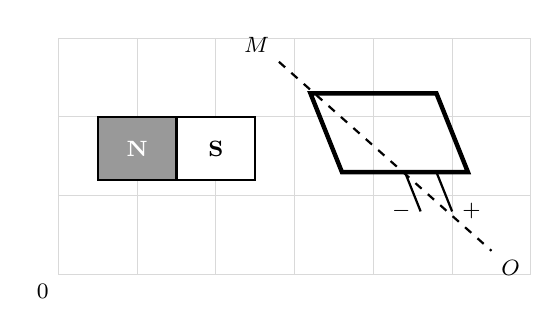
\begin{tikzpicture}[scale=1.0, every node/.style={font=\footnotesize}]
    \draw[xstep=1, ystep=1, gray!30, thin] (0,0) grid (6,3);
    
    % Полосовой магнит
    \draw[thick, black, fill=gray!80] (0.5,1.2) rectangle (1.5,2.0) node[pos=.5, white] {\textbf{N}};
    \draw[thick, black, fill=white] (1.5,1.2) rectangle (2.5,2.0) node[pos=.5] {\textbf{S}};
    
    % Ось MO
    \draw[dashed, black, thick] (2.8,2.7) -- (5.5,0.3);
    \node[above left] at (2.8,2.7) {$M$};
    \node[below right] at (5.5,0.3) {$O$};
    
    % Рамка (перспективный параллелограмм)
    \draw[ultra thick, black] (3.2,2.3) -- (4.8,2.3) -- (5.2,1.3) -- (3.6,1.3) -- cycle;
    
    % Выводы к источнику
    \draw[thick, black] (4.8,1.3) -- (5.0,0.8) node[right] {$+$};
    \draw[thick, black] (4.4,1.3) -- (4.6,0.8) node[left] {$-$};
    
    \node[below left] at (0,0) {0};
\end{tikzpicture}
\end{center}

\kim{21}
\end{taskbasic}
\answer{Рамка повернётся вокруг оси $MO$ и притянется к южному полюсу $S$ магнита}

% === ЗАДАЧА ===
% Тег: #ЭЛЕКТРОДИНАМИКА #МАГНЕТИЗМ #СИЛА_ЛОРЕНЦА #КИМ_12
\begin{taskbasic}[code={\label{task:elem_mag_particles_ratio_q2q_v2v}}]
Две частицы с зарядами $q_1 = q$ и $q_2 = 2q$ влетают в однородное магнитное поле перпендикулярно вектору магнитной индукции со скоростями $v_1 = v$ и $v_2 = 2v$ соответственно. Определите отношение модулей сил $\frac{F_1}{F_2}$, действующих на них со стороны магнитного поля.

\kim{12}
\end{taskbasic}
\answer{0,25}

% === ЗАДАЧА 1 ===
% Тег: #ЭЛЕКТРОДИНАМИКА #МАГНЕТИЗМ #СИЛА_ЛОРЕНЦА #КИМ_23
\begin{taskbasic}[code={\label{task:elem_mag_particle_charge_energy}}]
Заряженная частица с массой $m = 1{,}6 \cdot 10^{-25}\text{ кг}$ и зарядом $q$ движется по окружности радиусом $R = 0{,}4\text{ м}$ перпендикулярно линиям магнитной индукции однородного магнитного поля с индукцией $B = 0{,}5\text{ Тл}$. Кинетическая энергия частицы $W = 8 \cdot 10^{-14}\text{ Дж}$. Найдите заряд данной частицы, считая его положительным. Релятивистскими эффектами пренебречь. Ответ выразите в кулонах (Кл).

\kim{23}
\end{taskbasic}
\answer{$8\cdot 10^{-19}$}

% === ЗАДАЧА 2 ===
% Тег: #ЭЛЕКТРОДИНАМИКА #МАГНЕТИЗМ #СИЛА_ЛОРЕНЦА #КИМ_15
\begin{taskbasic}[code={\label{task:elem_mag_ion_field_reduction}}]
Ион натрия движется по окружности в однородном магнитном поле. Как изменятся сила, действующая на ион в магнитном поле, и частота его обращения, если, не меняя скорости иона, уменьшить модуль вектора индукции магнитного поля?

Для каждой величины определите соответствующий характер изменения:
1) увеличится
2) уменьшится
3) не изменится

\kim{15}
\end{taskbasic}
\answer{22}

% === ЗАДАЧА 3 ===
% Тег: #ЭЛЕКТРОДИНАМИКА #МАГНЕТИЗМ #СИЛА_АМПЕРА #НАКЛОННАЯ_ПЛОСКОСТЬ #КИМ_25
\begin{taskbasic}[code={\label{task:elem_mag_rod_inclined_plane}}]
Горизонтальный проводящий стержень прямоугольного сечения поступательно движется с ускорением $a = 1{,}5\text{ м/с}^2$ вверх по гладкой диэлектрической наклонной плоскости в вертикальном однородном магнитном поле (см. рисунок). Угол наклона плоскости $\alpha = 30^\circ$. Отношение массы стержня к его длине $\frac{m}{L} = 0{,}1\text{ кг/м}$. Модуль индукции магнитного поля $B = 0{,}3\text{ Тл}$. Определите силу тока $I$, протекающего по стержню. Сделайте рисунок с указанием сил, действующих на стержень. Ответ выразите в амперах (А).

\nopagebreak\smallskip
\begin{center}
\begin{tikzpicture}[scale=1.0, every node/.style={font=\footnotesize}]
    \draw[xstep=1, ystep=1, gray!30, thin] (0,0) grid (5,3);
    
    % Наклонная плоскость
    \draw[thick, black] (0.5,0.5) -- (4.5,2.5) -- (4.5,0.5) -- cycle;
    \draw (1.2,0.5) arc (0:26.56:0.7) node[pos=0.6, right] {$\alpha$};
    
    % Вектор индукции B (вертикально вверх)
    \draw[-{Stealth[scale=0.8]}, thick, black] (1.0,0.8) -- (1.0,2.6) node[above] {$\vec{B}$};
    
    % Стержень на плоскости
    \draw[thick, black, fill=white, rotate around={26.56:(2.2,1.35)}] (1.7,1.2) rectangle (2.7,1.5);
    
    % Ток I (стрелка на стержне)
    \draw[-{Stealth[scale=0.8]}, thick, black] (2.4,1.6) -- (1.8,1.3) node[above=2pt] {$I$};
    
    % Ускорение a (параллельно плоскости)
    \draw[-{Stealth[scale=0.8]}, thick, black] (2.8,1.9) -- (3.6,2.3) node[above left] {$\vec{a}$};
    
    \node[below left] at (0,0) {0};
\end{tikzpicture}
\end{center}

\kim{25}
\end{taskbasic}
\answer{2,5}
